%  LaTeX support: latex@mdpi.com 
%  For support, please attach all files needed for compiling as well as the log file, and specify your operating system, LaTeX version, and LaTeX editor.

%=================================================================
\documentclass[journal,article,submit,pdftex,moreauthors]{Definitions/mdpi} 
%---------
% pdftex
%---------
% The option pdftex is for use with pdfLaTeX. Remove "pdftex" for (1) compiling with LaTeX & dvi2pdf (if eps figures are used) or for (2) compiling with XeLaTeX.

%=================================================================
% MDPI internal commands - do not modify
\firstpage{1} 
\makeatletter 
\setcounter{page}{\@firstpage} 
\makeatother
\pubvolume{1}
\issuenum{1}
\articlenumber{0}
\pubyear{2023}
\copyrightyear{2023}
%\externaleditor{Academic Editor: Firstname Lastname}
\datereceived{ } 
\daterevised{ } % Comment out if no revised date
\dateaccepted{ } 
\datepublished{ } 
%\datecorrected{} % For corrected papers: "Corrected: XXX" date in the original paper.
%\dateretracted{} % For corrected papers: "Retracted: XXX" date in the original paper.
\hreflink{https://doi.org/} % If needed use \linebreak
%\doinum{}
%\pdfoutput=1 % Uncommented for upload to arXiv.org

%=================================================================
% Add packages and commands here. The following packages are loaded in our class file: fontenc, inputenc, calc, indentfirst, fancyhdr, graphicx, epstopdf, lastpage, ifthen, float, amsmath, amssymb, lineno, setspace, enumitem, mathpazo, booktabs, titlesec, etoolbox, tabto, xcolor, colortbl, soul, multirow, microtype, tikz, totcount, changepage, attrib, upgreek, array, tabularx, pbox, ragged2e, tocloft, marginnote, marginfix, enotez, amsthm, natbib, hyperref, cleveref, scrextend, url, geometry, newfloat, caption, draftwatermark, seqsplit
% cleveref: load \crefname definitions after \begin{document}

%=================================================================
% Please use the following mathematics environments: Theorem, Lemma, Corollary, Proposition, Characterization, Property, Problem, Example, ExamplesandDefinitions, Hypothesis, Remark, Definition, Notation, Assumption
%% For proofs, please use the proof environment (the amsthm package is loaded by the MDPI class).

%=================================================================
% Full title of the paper (Capitalized)
\Title{Driver Monitoring System with Arduino Nano 33 BLE}

% MDPI internal command: Title for citation in the left column
\TitleCitation{Title}

% Author Orchid ID: enter ID or remove command
\newcommand{\orcidauthorA}{0000-0000-0000-000X} % Add \orcidA{} behind the author's name
%\newcommand{\orcidauthorB}{0000-0000-0000-000X} % Add \orcidB{} behind the author's name

% Authors, for the paper (add full first names)
\Author{Harsh Gangwar, Rohan khaire, Joel Eliston and Rohit Menon} 

%\longauthorlist{yes}

% MDPI internal command: Authors, for metadata in PDF
\AuthorNames{Harsh Gangwar, Rohan khaire, Joel Eliston and Rohit Menon}

% MDPI internal command: Authors, for citation in the left column
\AuthorCitation{Gangwar, H.; Khaire, R.; Eliston, J; Menon R.}
% If this is a Chicago style journal: Lastname, Firstname, Firstname Lastname, and Firstname Lastname.

% Affiliations / Addresses (Add [1] after \address if there is only one affiliation.)
\address{%
$^{1}$ \quad hgangwar@asu.edu\\
$^{2}$ \quad rkhaire@asu.edu\\
$^{3}$ \quad jeliston@asu.edu\\
$^{4}$ \quad rmenon12@asu.edu}
% The commands \thirdnote{} till \eighthnote{} are available for further notes

%\simplesumm{} % Simple summary

%\conference{} % An extended version of a conference paper

% Abstract (Do not insert blank lines, i.e. \\) 
\abstract{This paper presents the development of a Driver Monitoring System (DMS) utilizing the Arduino Nano 33 BLE and an integrated camera module. The system focuses on real-time monitoring of the driver's behavior using Convolutional Neural Networks (CNNs). The Arduino Nano 33 BLE serves as a compact and low-power microcontroller and its camera captures real-time images of the driver. The CNN model is employed to analyze facial expressions, eye movements, and head gestures, providing a comprehensive assessment of the driver's attention and alertness levels. The system aims to enhance road safety by detecting signs of drowsiness or distraction, and subsequently alerting the driver in real-time. The utilization of Arduino Nano 33 BLE ensures a cost-effective and easily deployable solution, making it suitable for integration into various vehicles. The real-time CNN-based analysis enables quick and accurate identification of potential driver safety risks, contributing to a proactive approach in preventing accidents caused by driver-related factors. The proposed Driver Monitoring System offers a versatile and accessible solution for enhancing driver safety through continuous monitoring, paving the way for the integration of advanced driver-assistance systems in a wide range of vehicles..}

% Keywords
\keyword{Deep learning; Driver fatigue detect; Embedded system; Image processing} 


%%%%%%%%%%%%%%%%%%%%%%%%%%%%%%%%%%%%%%%%%%
\begin{document}

%%%%%%%%%%%%%%%%%%%%%%%%%%%%%%%%%%%%%%%%%%
%\setcounter{section}{0} %% Remove this when starting to work on the template.

\section{Introduction}

Our research addresses a significant gap in the current landscape where high-end Python or Java-based products dominate the industry. The primary goal is to democratize access to advanced technology by creating a cost-effective and affordable solution accessible to a broader audience. Focusing on low-cost microcontrollers, our work explores the boundaries of complexity in model design, the scalability of label consideration, and the identification of the most suitable CNN architecture for this application.

In this pursuit, we aim to redefine the parameters of feasibility and effectiveness in the realm of cost-effective solutions. By pushing the boundaries of what low-cost microcontrollers can achieve, we seek to determine the optimal balance between affordability and performance. Our research delves into the intricacies of deploying complex models in resource-constrained environments and addresses critical questions about the number of labels that can be accommodated. Through this investigation, we aspire to provide comprehensive answers that contribute to the development of economically viable solutions, making advanced technology accessible to a wider demographic and fostering innovation in the integration of affordable, high-performance systems.
%%%%%%%%%%%%%%%%%%%%%%%%%%%%%%%%%%%%%%%%%%
\section{Related Work}

The current state of the art in monitoring systems includes noteworthy developments by industry leaders such as NXP Semiconductor and Qualcomm, both showcasing advanced Driver Monitoring Systems (DMS). NXP's system is designed around five features, including Yawning, Drinking, Smoking, Eyes closed, and On a call. Meanwhile, Qualcomm's DMS, presented at CVPR23, exhibits a broader capability, detecting activities such as Calling, Drinking, Smoking, Yawning, Hands off steering wheel, Arm out windows, and Looking direction.

However, a literature gap emerges concerning cost-effective solutions and the integration of such advanced monitoring capabilities into low-cost microcontrollers. Notably, existing research has explored Embedded systems using Nvidia Jetson Nano and Jetson Tk1 for DMS, with a focus on detecting Eye closing and yawning.

In this context, our work aims to bridge this gap by bringing the capabilities of sophisticated monitoring systems to the accessible and cost-effective realm of Arduino Nano 33 BLE. This shift addresses the need for affordable solutions without compromising the intricacies of detection, expanding the possibilities for implementing robust Driver Monitoring Systems in a wider range of applications and environments.

\section{System Design}
In crafting our system design, our approach is centered on a thorough exploration of different system architectures to gauge their effectiveness. Currently, we are in the initial phase of establishing benchmark algorithms/models to assess the performance of diverse architectures during experimentation.

For model training, we have devised a custom Convolutional Neural Network (CNN) architecture capable of recognizing 10 distinct classes as specified in the dataset. In addition to our custom CNN, we implemented transfer learning using pre-trained models like MobileNetV3 and DenseNet. Leveraging the transfer learning technique, we fine-tuned these models for our specific application.

Training was conducted on a local system equipped with an RTX 3070 GPU boasting 8GB of VRAM, ensuring efficient processing. The training results showcase the efficacy of our models, with the custom CNN achieving a training accuracy of 97\% and a validation accuracy of 96.5\%. MobileNetV3 exhibited a training accuracy of 98.3\% and a validation accuracy of 96.7\%, while DenseNet achieved a training accuracy of 93.3\% and a validation accuracy of 92.1\%.

As our work progresses, this foundation will guide us in selecting the most suitable system architecture for real-time execution on embedded devices, with a focus on optimizing the model for efficient and effective performance.
%%%%%%%%%%%%%%%%%%%%%%%%%%%%%%%%%%%%%%%%%%



\section{Evaluation Approach}

In our exploration of driver monitoring system architectures, we present model accuracy and loss plots for three distinct models: Custom CNN, MobileNetV3, and DenseNet. These visualizations offer insights into the training process, showcasing the performance of each architecture.

\subsection{Figures, Tables and Schemes}
\begin{figure}[H]
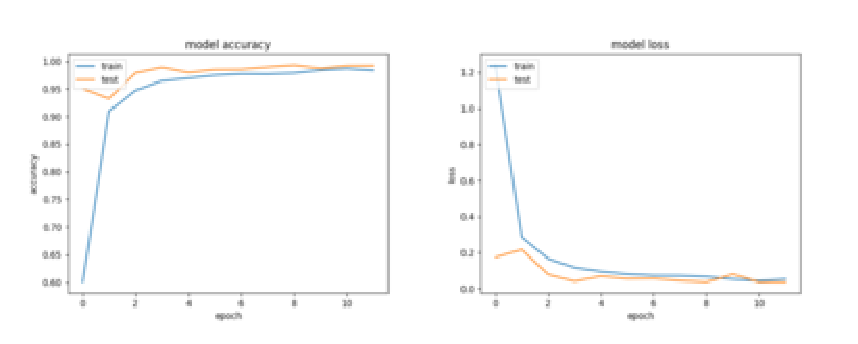
\includegraphics[width=10.5 cm]{customCNN}
\caption{Custom CNN: (\textbf{a}) Model Accuracy. (\textbf{b}) Model Loss.\label{fig1}}
\end{figure}  
\begin{figure}[H]
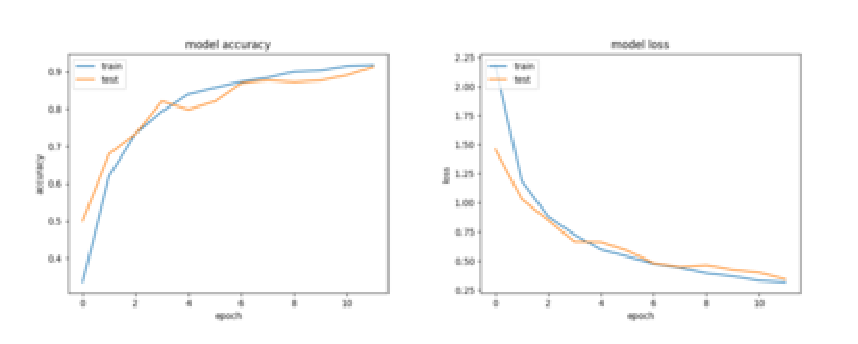
\includegraphics[width=10.5 cm]{DenseNet}
\caption{DenseNet: (\textbf{a}) Model Accuracy. (\textbf{b}) Model Loss.\label{fig2}}
\end{figure}  
\begin{figure}[H]
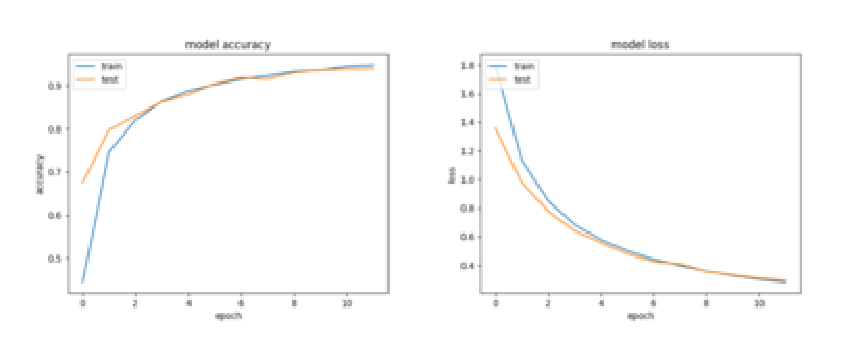
\includegraphics[width=10.5 cm]{mobileNET_V3}
\caption{MobileNET V3: (\textbf{a}) Model Accuracy. (\textbf{b}) Model Loss.\label{fig3}}
\end{figure}
%%%%%%%%%%%%%%%%%%%%%%%%%%%%%%%%%
\section{Experimentation Process}

\subsection{Arduino}
Initially, we adapted various models (including a custom Convolutional Neural Network (CNN), MobileNetV3, and DenseNet) to ensure compatibility with the Arduino platform. Subsequently, we modified the example code, specifically the one labeled "person detection" in Harvard Tiny ML, to repurpose it as a driver detection system.

During the course of the experiment, we encountered a challenge when our model turned out to be too large for the Arduino's capacity. To address this issue, we redesigned the model, adjusting the image size to 96x96 pixels and converting it to grayscale. This alteration allowed us to fit the model within the dynamic memory constraints of the Arduino. However, a new problem arose as the Arduino consistently generated the output "Invoke failed." We suspect that the model architecture we created differs from the one employed by Harvard Tiny ML. Despite extensive online research, we were unable to locate information on the specific model they utilized.

Faced with this roadblock, we made the decision to switch to a BeagleBone Black microcontroller. The BeagleBone's capability to operate its own Linux operating system provided us with confidence that our project could be successfully executed on this platform.

\subsection{BeagleBone}
To employ the BeagleBone, our initial step involved installing all the necessary libraries, with a particular emphasis on OpenCV. Initially, we attempted to build OpenCV directly on the BeagleBone. However, due to its constrained computing resources, we encountered an out-of-memory error during the build process. Subsequently, we opted for a cross-compilation approach, using a Docker image of Debian that emulates the BeagleBone's architecture (ARMHF). After successful compilation, we transferred the OpenCV library to the BeagleBone, effectively integrating it into the platform.

In our attempts to capture live images from a camera, we encountered a challenge when attempting to connect a webcam directly to the BeagleBone, as the microcontroller lacked the power to support it. To address this limitation, we explored an alternative approach by attempting to access the laptop's webcam through the BeagleBone. Unfortunately, we encountered permission issues that prevented successful access. Ultimately, we devised a solution using a Python script to transmit the webcam feed through a socket, paired with another Python script on the BeagleBone to receive and display the live images. This workaround allowed us to successfully obtain and display live images on the BeagleBone.

Now, our project involves the use of two Python scripts to facilitate its operation.

The first script is responsible for capturing live video as bytes from the webcam connected to the laptop. Subsequently, it transmits this data to the BeagleBone, establishing a seamless communication channel between the devices.

The second script is designed to receive the transmitted data on the BeagleBone. It performs the essential task of converting the received bytes back into images. These images are then fed into our model, enabling it to generate predictions based on the input data.

This dual-script setup ensures the effective execution of our project, allowing for the seamless transfer and processing of live video data from the laptop to the BeagleBone, ultimately resulting in accurate predictions from our model
%%%%%%%%%%%%%%%%%%%%%%%%%%%%%%%
\subsection{Neural Network Structure}

Our neural network was trained using the MobileNetV1 architecture, utilizing pre-trained weights from ImageNet. To optimize memory efficiency for embedded devices, we applied a width factor of 0.25 during training. As a result, the model size was constrained to 875 kilobytes (kbs). Subsequently, to further enhance its suitability for embedded systems, we performed full 8-bit integer quantization on our original 32-bit float model. The quantized model, now represented in 8-bit integer format, was successfully compressed to a size of 300 kilobytes (kbs). This reduction in size ensures the efficient deployment of the neural network on resource-constrained devices while maintaining its predictive capabilities.

\begin{figure}[H]
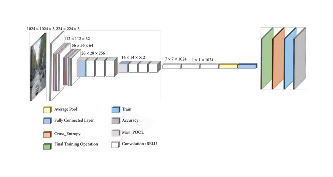
\includegraphics[width=10.5 cm]{architecture_MobileNet}
\caption{MobileNet V1 Architecture\label{fig1}}
\end{figure}

\subsection{Results }
Ultimately, we opted to adhere to the MobileNet-derived model, as the other models proved to be incompatible. The achieved results demonstrate a validation accuracy of approximately 85\% and a validation loss of around 0.18.
\subsection{Figures, Tables and Schemes}
\begin{figure}[H]
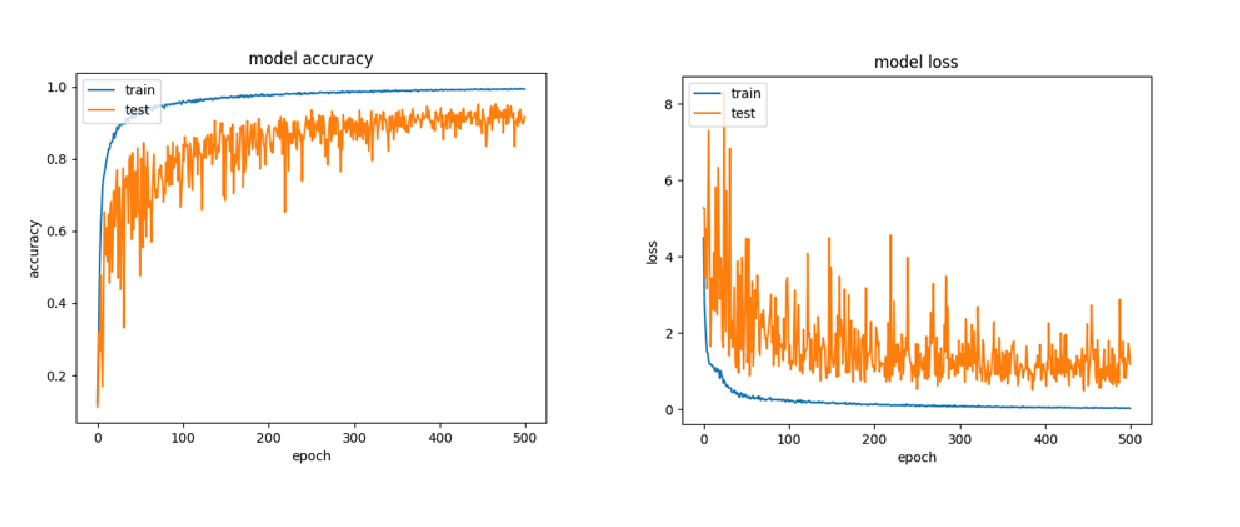
\includegraphics[width=10.5 cm]{model.eps}
\caption{MobileNetV1: (\textbf{a}) Model Accuracy. (\textbf{b}) Model Loss.\label{fig1}}
\end{figure} 


For the specific requirements of our project, which involves binary classification into two labels (Alert and Not Alert), we made the following interpretation of the model's predictions: If the model predicted class "c0," it was interpreted as Alert, whereas predictions falling into any other classes (c1 – c9) were categorized as Not Alert. This simplified classification approach effectively met the needs of our project while maintaining a satisfactory level of accuracy.



%%%%%%%%%%%%%%%%%%%%%%%%%%%%%


\reftitle{References}

% Please provide either the correct journal abbreviation (e.g. according to the “List of Title Word Abbreviations” http://www.issn.org/services/online-services/access-to-the-ltwa/) or the full name of the journal.
% Citations and References in Supplementary files are permitted provided that they also appear in the reference list here. 

%=====================================
% References, variant A: external bibliography
%=====================================
%\bibliography{your_external_BibTeX_file}

%=====================================
% References, variant B: internal bibliography
%=====================================
\begin{thebibliography}{999}
% Reference 1
\bibitem[Reddy (2017)]{IEEE}
B. Reddy, Y. -H. Kim, S. Yun, C. Seo and J. Jang, "Real-Time Driver Drowsiness Detection for Embedded System Using Model Compression of Deep Neural Networks," 2017 IEEE Conference on Computer Vision and Pattern Recognition Workshops (CVPRW), Honolulu, HI, USA, 2017, pp. 438-445, doi: 10.1109/CVPRW.2017.59. (Accessed: 08 November 2023). 
% Reference 2
\bibitem[Esra(2023)]{ScienceDirect}
Esra Civik, Ugur Yuzgec, Real-time driver fatigue detection system with deep learning on a low-cost embedded system, Microprocessors and Microsystems, Volume 99, 2023, 104851, ISSN 0141-9331, https://doi.org/10.1016/j.micpro.2023.104851 (https://www.sciencedirect.com/science
/article/pii/S0141933123000972)(Accessed: 08 November 2023). 


% If authors have biography, please use the format below
%\section*{Short Biography of Authors}
%\bio
%{\raisebox{-0.35cm}{\includegraphics[width=3.5cm,height=5.3cm,clip,keepaspectratio]{Definitions/author1.pdf}}}
%{\textbf{Firstname Lastname} Biography of first author}
%
%\bio
%{\raisebox{-0.35cm}{\includegraphics[width=3.5cm,height=5.3cm,clip,keepaspectratio]{Definitions/author2.jpg}}}
%{\textbf{Firstname Lastname} Biography of second author}

% For the MDPI journals use author-date citation, please follow the formatting guidelines on http://www.mdpi.com/authors/references
% To cite two works by the same author: \citeauthor{ref-journal-1a} (\citeyear{ref-journal-1a}, \citeyear{ref-journal-1b}). This produces: Whittaker (1967, 1975)
% To cite two works by the same author with specific pages: \citeauthor{ref-journal-3a} (\citeyear{ref-journal-3a}, p. 328; \citeyear{ref-journal-3b}, p.475). This produces: Wong (1999, p. 328; 2000, p. 475)

%%%%%%%%%%%%%%%%%%%%%%%%%%%%%%%%%%%%%%%%%%
%% for journal Sci
%\reviewreports{\\
%Reviewer 1 comments and authors’ response\\
%Reviewer 2 comments and authors’ response\\
%Reviewer 3 comments and authors’ response
%}
%%%%%%%%%%%%%%%%%%%%%%%%%%%%%%%%%%%%%%%%%%
%\end{adjustwidth}
\end{document}

